\newpage
\section{Pseudo-Spectral Time Domain Method}
The Fourier Pseudo-spectral Time Domain (PSTD) Method is a numerical method that can be used for solving partial differential equations in a similar way to the FDTD method. The advantage of this method is that differentiation occurs in the frequency domain, using the computational speed of performing a discrete Fourier transform to give fast frequency domain differentiation and differentiation with higher order accuracy than the FDTD method~\cite{Hornikx2016}. In this chapter we will discuss the application of the PSTD method to the acoustic wave equation, including the use of empirical partially absorbing boundary conditions and the perfectly matched layer(PML).

\subsection{A Background to the Pseudo-Spectral Time Domain Method}
The PSTD method is of a branch of spectral methods that are useful for solving some hyperbolic partial differential equations. Use of spectral differentiation for computational fluid dynamics modelling was first proposed by Orszag~\cite{Orszag1971}, and was further expanded by Kriess and Oliger~\cite{Kreiss1972}. Fourier Pseudospectral methods have been advanced considerably since then, and have found applications in weather prediction, particle physics, electromagnetics and acoustics. More recently Trefethen~\cite{Trefethen2000} presented a classic text showcasing both the power of spectral methods, and how simply they could be implemented. The Fourier PSTD method used in this study is advanced from that presented by Angus and Caunce ~\cite{Angus2010}, with expansion into 2 and 3 dimensions and implementation of partially absorbing boundary conditions. 

\subsection{Block Diagram}
The basic block diagram of a program for solving the the acoustic PSTD method is very similar to the FDTD Method. Below is a block diagram of the steps for solving one time step of the 2D PSTD method:\\

% Define block styles
\tikzstyle{decision} = [diamond, draw, fill=blue!20, 
    text width=4.5em, text badly centered, node distance=3cm, inner sep=0pt]
\tikzstyle{block} = [rectangle, draw, fill=blue!20, 
    text width=5em, text centered, rounded corners, minimum height=4em]
\tikzstyle{line} = [draw, -latex']
\tikzstyle{cloud} = [draw, ellipse,fill=red!20, node distance=3cm,
    minimum height=2em]
\begin{center}
\begin{tikzpicture}[node distance = 2cm, auto]
    % Place nodes
    \node [block] (init) {Start (t)};
    \node [block, below of=init] (fftp) {FFT $p$};
    \node [block, below left of=fftp] (diffx) {Differentiate $\textit{F}(p)$ in x direction};
    \node [block, below right of=fftp] (diffy) {Differentiate $\textit{F}(p)$ in y direction};
    \node [block, below of=diffx] (ifftxh) {IFFT $\hat{u}_x$ in x direction};
    \node [block, below of=diffy] (ifftyh) {IFFT $\hat{u}_y$ in y direction};
    \node [block, below of=ifftxh] (evalux) {Update $u_x$ with $\hat{u}_x$};
    \node [block, below of=ifftyh] (evaluy) {Update $u_y$ with $\hat{u}_y$};
    \node [block, below of=evalux] (fftux) {FFT $u_x$};
    \node [block, below of=evaluy] (fftuy) {FFT $u_y$};
    \node [block, below of=fftux] (diffux) {Differentiate $\textit{F}u_x$};
    \node [block, below of=fftuy] (diffuy) {Differentiate $\textit{F}u_y$};
    \node [block, below of=diffux] (ifftuhx) {IFFT $\hat{u}_x$};
    \node [block, below of=diffuy] (ifftuhy) {IFFT $\hat{u}_y$};
    \node [block, below right of=ifftuhx] (evaluatep) {Update $p$ with $\hat{u}_x$ and $\hat{u}_y$};
    \node [block, below of=evaluatep] (source) {add source terms};
    \node [block, below of=source] (next) {$t = t + \delta t$};
    % Draw edges
    \path [line] (init) -- (fftp);
    \path [line] (fftp) -- (diffx);
    \path [line] (fftp) -- (diffy);
    \path [line] (diffx) -- (ifftxh);
    \path [line] (diffy) -- (ifftyh);
    \path [line] (ifftxh) -- (evalux);
    \path [line] (ifftyh) -- (evaluy);
    \path [line] (evalux) -- (fftux);
    \path [line] (evaluy) -- (fftuy);
    \path [line] (fftux) -- (diffux);
    \path [line] (fftuy) -- (diffuy);
    \path [line] (diffux) -- (ifftuhx);
    \path [line] (diffuy) -- (ifftuhy);
    \path [line] (ifftuhx) -- (evaluatep);
    \path [line] (ifftuhy) -- (evaluatep);
    \path [line] (evaluatep) -- (source);
    \path [line] (source) -- (next);
\end{tikzpicture}                                             
\end{center}
\subsection{The Pseudospectral Time Domain Method Applied To The Wave Equation}

The acoustic wave equation has been previously defined with two resolving parts:\\
\begin{equation}
\frac{\delta^2 p}{\delta t^2} = \frac{1}{c^2} \frac{\delta^2 p}{\delta t^2}\\
\end{equation}
\begin{equation}
\frac{\delta^2 u}{\delta t^2} = \frac{1}{c^2} \frac{\delta^2 u}{\delta t^2}\\
\end{equation}
Applying a continuous time Euler solving method to the above relationship with respect to space brings the following:\\
\begin{equation}
\rho_0 \frac{\delta}{\delta x}\left[\frac{\delta u}{\delta t}\right] =\frac{1}{c^2} \frac{\delta ^2 p}{\delta t^2} \\
\end{equation}
Implementing a discrete time and space version of this equation using an FDTD scheme yields:\\
\begin{equation}
u^{t + \frac{\delta t}{2}}_{x} = u^{t - \frac{\delta t}{2}}_{x} - \frac{\delta t}{\rho \delta x} \left[p^{t}_{x + \frac{\delta x}{2}} - p^{t}_{x - \frac{\delta x}{2}}\right]\\
\end{equation}
\begin{equation}
p^{t + \frac{\delta t}{2}}_{x} = p^{t - \frac{\delta t}{2}}_{x} - \frac{c^2 \rho \delta t}{\delta x} \left[u^{t}_{x + \frac{\delta x}{2}} - u^{t}_{x - \frac{\delta x}{2}}\right]\\
\end{equation}
The PSTD method applies differentiation in the frequency or $ \textit{k} space$ domain. This can be represented as:\\
\begin{equation}
u^{t + \frac{\delta t}{2}}_{x} = u^{t - \frac{\delta t}{2}}_{x} - \frac{\delta t}{\rho \delta x} \textbf{\textit{F}}^{-1}\left(\epsilon \textbf{\textit{F}}\left[p^{t}_{x}\right] \right)\\
\end{equation}
\begin{equation}
p^{t + \frac{\delta t}{2}}_{x} = p^{t - \frac{\delta t}{2}}_{x} - \frac{c^2 \rho \delta t}{\delta x} \textbf{\textit{F}}^{-1}\left( \epsilon \textbf{\textit{F}} \left[ u^{t}_{x} \right] \right)\\
\end{equation}
Where $\textbf{\textit{F}}$ represents the forward and $\textbf{\textit{F}}^{-1}$ the inverse Fourier Transforms respectively, and $\epsilon$ is a differentiating function representing:\\
\begin{equation}
\textbf{JK}_N \exp^{-jk_N\frac{\delta x}{2}}\\
\end{equation}
Which is the impulse response of a differentiating function in the complex domain, where N is the 1D size of the domain in the dimension of interest i.e. each dimension requires a differentiator function. In the 2D and 3D implementation of this method, extra velocity terms are added to handle the differentiation of directionally dependent terms:\\
\begin{equation}
u^{t + \frac{\delta t}{2}}_{x} = u^{t - \frac{\delta t}{2}}_{x} - \frac{\delta t}{\rho \delta x} \textbf{\textit{F}}^{-1}\left(\epsilon \textbf{\textit{F}}\left[p^{t}_{x}\right] \right)\\
\end{equation}
\begin{equation}
u^{t + \frac{\delta t}{2}}_{y} = u^{t - \frac{\delta t}{2}}_{y} - \frac{\delta t}{\rho \delta y} \textbf{\textit{F}}^{-1}\left(\epsilon \textbf{\textit{F}}\left[p^{t}_{y}\right] \right)\\
\end{equation}
\begin{equation}
u^{t + \frac{\delta t}{2}}_{z} = u^{t - \frac{\delta t}{2}}_{z} - \frac{\delta t}{\rho \delta z} \textbf{\textit{F}}^{-1}\left(\epsilon \textbf{\textit{F}}\left[p^{t}_{z}\right] \right)\\
\end{equation}
\begin{equation}
p^{t + \frac{\delta t}{2}}_{xyz} = p^{t - \frac{\delta t}{2}}_{xyz} - \frac{c^2 \rho \delta t}{\delta x} \textbf{\textit{F}}^{-1}\left( \epsilon \textbf{\textit{F}} \left[ u_x^{t} \right] \right) - \frac{c^2 \rho \delta t}{\delta y} \textbf{\textit{F}}^{-1}\left( \epsilon \textbf{\textit{F}} \left[ u_y^{t} \right] \right) - \frac{c^2 \rho \delta t}{\delta z} \textbf{\textit{F}}^{-1}\left( \epsilon \textbf{\textit{F}} \left[ u_z^{t} \right] \right)\\
\end{equation}
The figure below shows a 2D matrix used for differentiation on a 2D simulation in one direction:\\
\begin{figure}[H]
\centering
  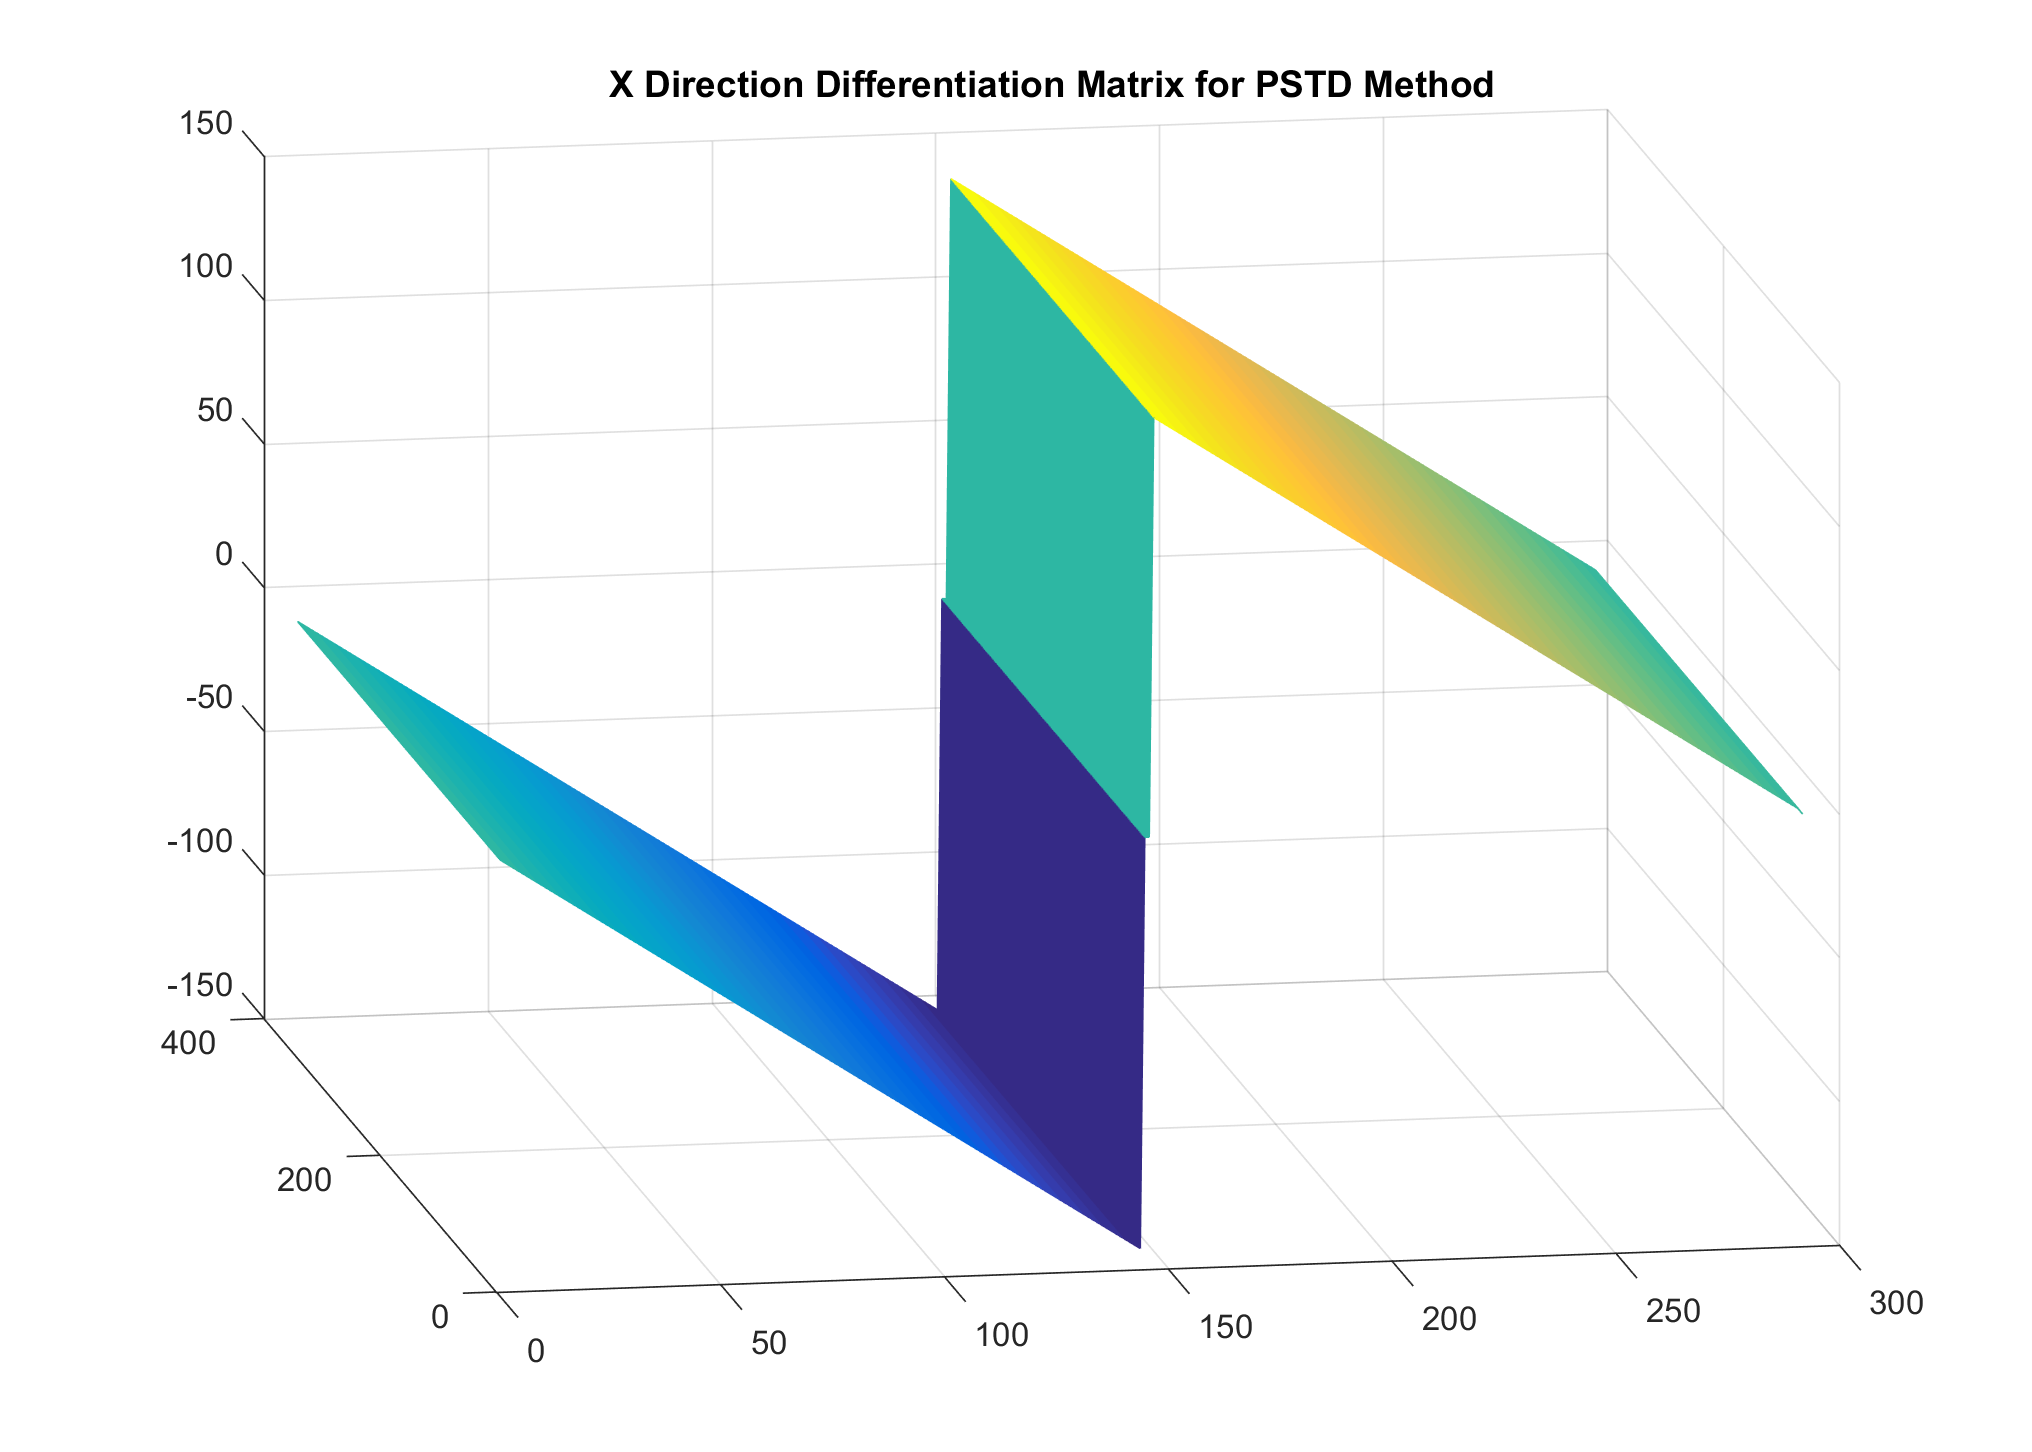
\includegraphics[width=0.75\textwidth]{./graphics/pstd2ddiffmatrix.png}
  \caption{2D Differentiation Matrix in 1 Direction for a PSTD Simulation}
\end{figure}

A Matlab function for solving 1 time step of the PSTD method is given below:\\
\lstinputlisting[language=Matlab]{../Matlab/PSTD/PSTD3Dfun.m}
%\lstinputlisting[language=Matlab]{../Matlab/SFDTD/SPARSEfun2DC.m}

\subsection{Absorbing Boundary Conditions}
The Fourier PSTD is performs well for problems with smoothly varying properties, but this method suffers from Gibbs phenomenon as the domain is periodic and has discontinuity at its boundaries i.e. it is not infinitely long. This is manifested as aliasing in the domain. A way to reduce this aliasing is to increase the area of the domain and implement a perfectly matched layer (PML). A PML is a totally absorbing boundary condition that absorbs waves travelling into it without causing reflection due to impedance mismatching, as opposed to a more simple boundary condition such as Dirchlet (fixed) that will cause reflections~\cite{Rumpf2012a}. The PML was first developed for Maxwell's Equations in Computational Electromagnetics by Berenger~\cite{Berenger1994}, and was quickly developed for other applications such as acoustic FDTD and FE~\cite{Liu1997}.\\

Three predominant types of PML available are the split field PML, Uniaxial PML and the Convolutional PML. For the sake of time saving and simplicity, the uniaxial PML is implemented in this study as is implemented in the source literature~\cite{Angus2010}. The PML is implemented as a matrix with the same dimensions as the domain, which has been extended in each dimension by the number of cells matching the desired depth of the PML $N_{pml}$. In the PML region, the value of the PML contribution to the $p$ and $u$ update equations $\sigma$, reduces in value from 1 to 0 towards the final boundary of the domain, continuously and smoothly impeding acoustic waves in any direction within the PML causing no reflection of waves from the PML back into the domain main domain.\\
 
The modified 1D update equation for this is as follows:\\
\begin{equation}
u^{t + \frac{\delta t}{2}}_{x} = u^{t - \frac{\delta t}{2}}_{x} \sigma_a - \frac{\delta t}{\rho \delta x} \sigma_b \textbf{\textit{F}}^{-1}\left(\epsilon \textbf{\textit{F}}\left[p^{t}\right] \right)\\
\end{equation}
\begin{equation}
p^{t + \frac{\delta t}{2}}_{x} = p^{t - \frac{\delta t}{2}}_{x} \sigma_a - \frac{c^2 \rho \delta t}{\delta x} \sigma_b \textbf{\textit{F}}^{-1}\left( \epsilon \textbf{\textit{F}} \left[ u^{t} \right] \right)\\
\end{equation}
Where:\\
\begin{equation}
\begin{aligned}
\sigma_a & = \frac{1-a}{1+a} \\
\sigma_b & = \frac{1}{1 + a} \\
d & = PML Depth\\
N & = Total Array Length \\
i & = 1,2... N-1\\
i < d \quad a & = \frac{1}{3} \left( \frac{i}{d} \right)^3\\
d < i < N - d \quad a & = 0\\
i > N-d \quad a & = \frac{1}{2} \left( \frac{N - i}{d} \right) ^3 \\ 
\end{aligned}
\end{equation}

As the maximum number in the matrix is 1, a multidimensional implementation of the PML regions involved creating orthogonal arrays of these 1D sections and applying an average summation of the regions values. Generating 2D PML coefficients involves summing 2 orthogonal 2D $N_x N_y $ matrices using a least squares method. Generating a 3D matrix of PML coefficients involved creating 3 3D $N_x N_y N_z $ matrices, with sets of 1D coefficient arrays in each direction. These three orthogonal matrices are summed and divided by the number of matrices. An example of the values of PML coefficients in a 2D simulation can be found below:\\
\begin{figure}[H]
\centering
  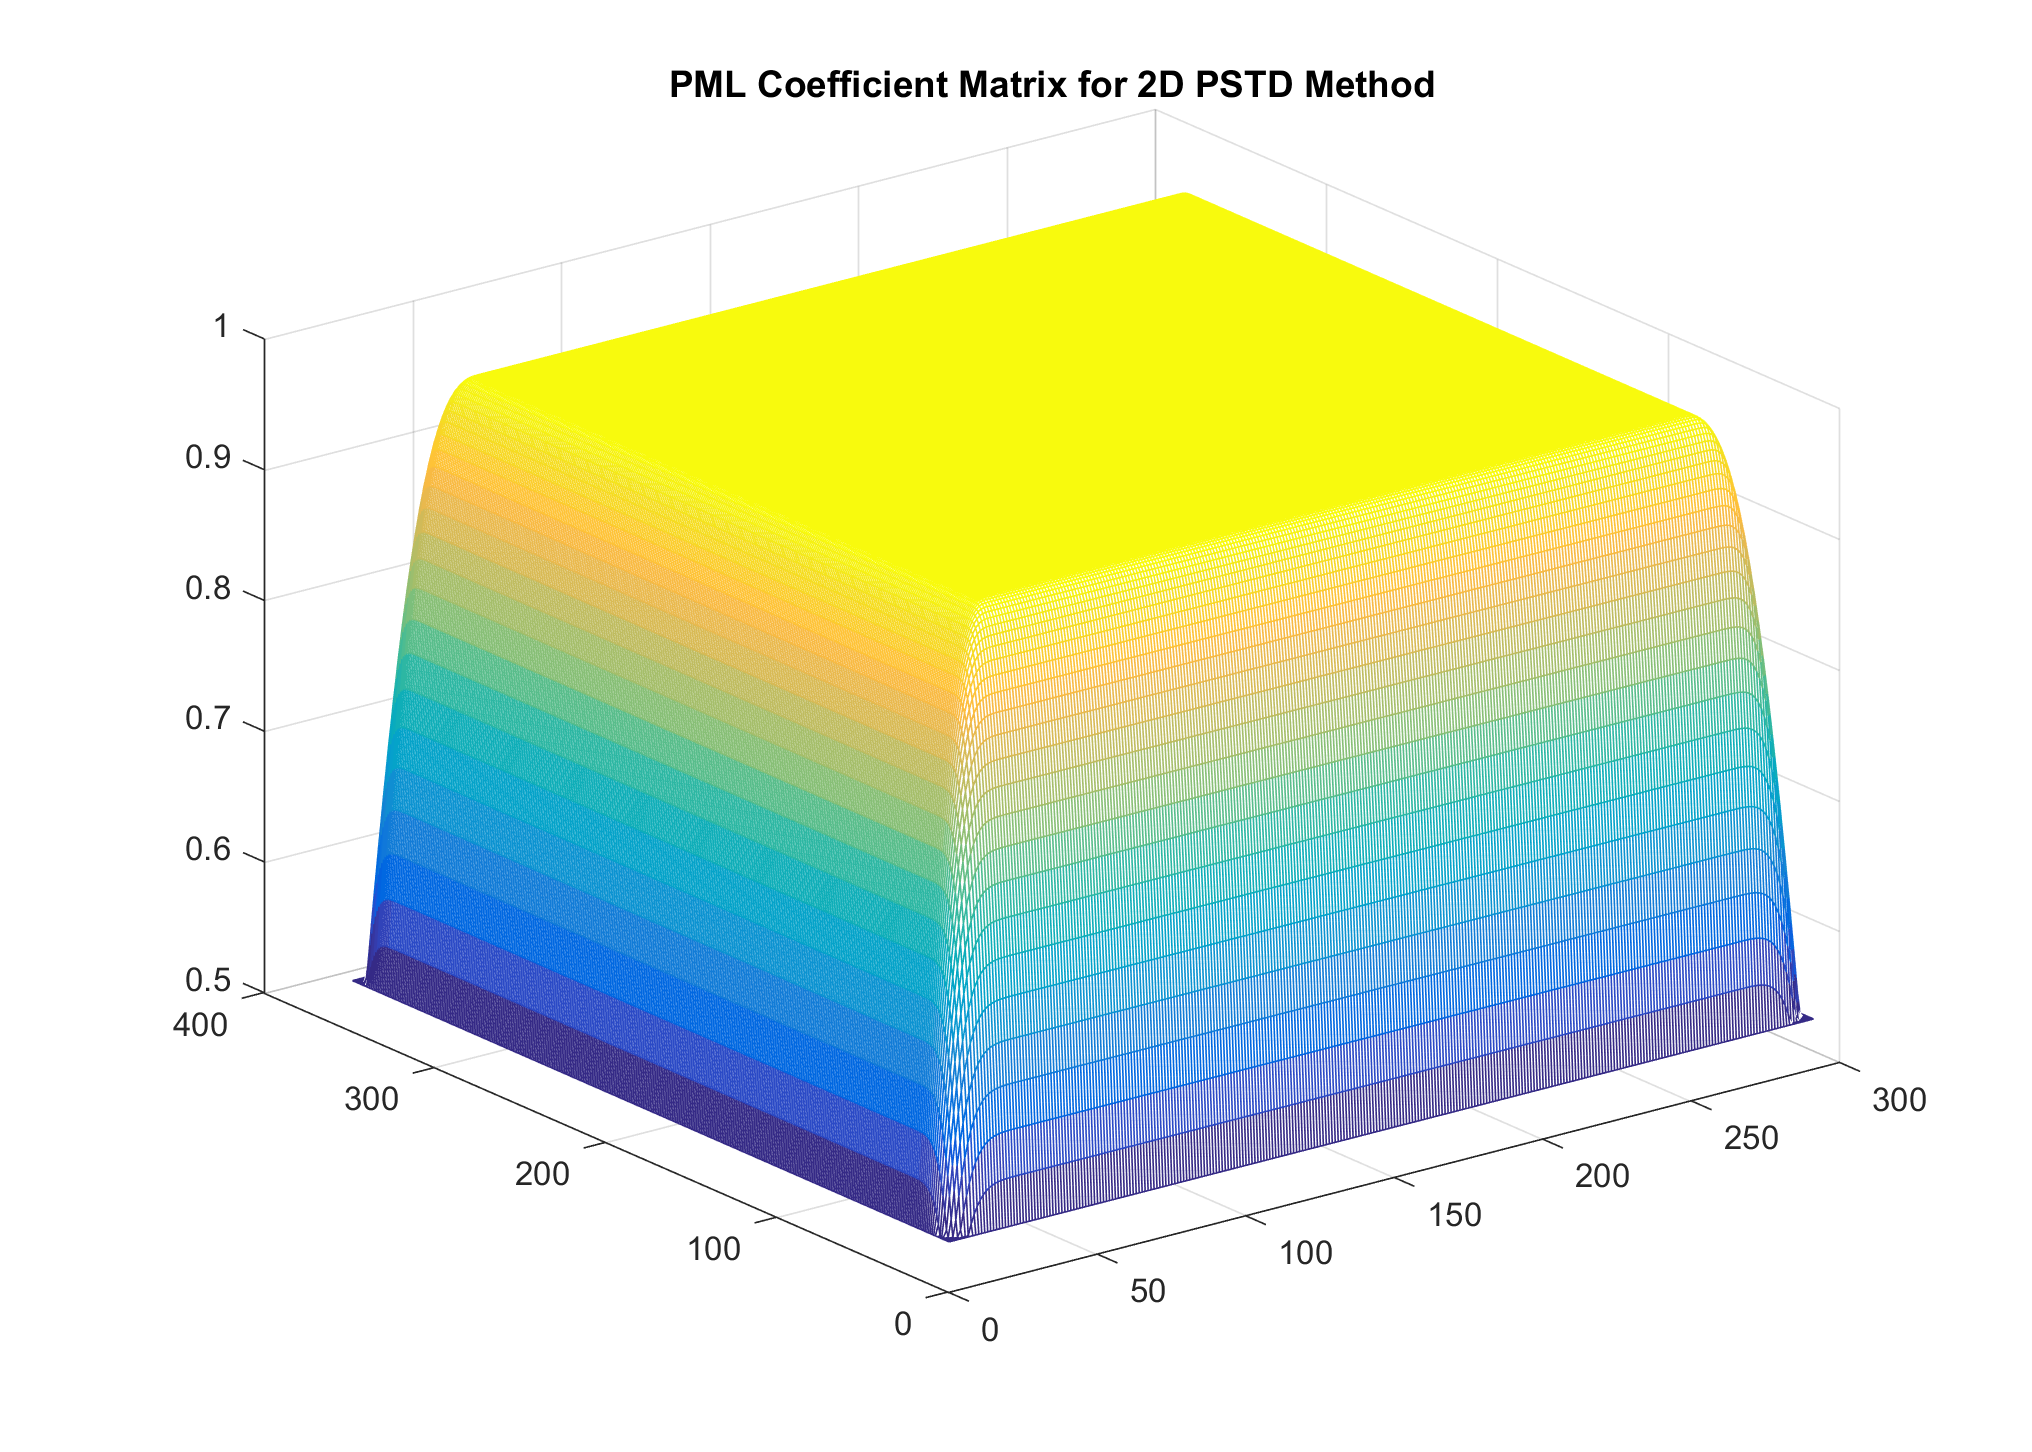
\includegraphics[width=0.75\textwidth]{./graphics/pstd2dpmlmatrix.png}
  \caption{PSTD 2D PML Coefficient Matrix}
\end{figure}


\subsection{Partially Absorbing Boundary Conditions}
Partially absorbing boundary conditions for PSTD are implemented in this study using the methods explored by Spa \textit{et al.}~\cite{Spa2011}, where a real and normalised value can be defined and used as a frequency independent absorption coefficient for boundary impedance setting. This method applies a weighting to the relationship between pressure and velocity at the grid boundaries, reflecting and passing a proportion of energy.\\

This boundary handling method uses the principal of acoustic impedance $Z$ mentioned previously, to absorb or reflect at the imposed boundary of the domain. The relationship between boundary coefficient $\xi$, and acoustic impedance is as follows:

\begin{equation}
\begin{aligned}
\textrm{For} \xi \leq 1: & \\
\xi = \frac{Z / (\rho c)}{S + Z / (\rho c) - Z S / (\rho c)}\\
\textrm{For} \xi \geq 1: & \\
\xi = Z S / (\rho c) - S + 1\\
\end{aligned}
\end{equation}
Where $S$ is the CFL coefficient of the simulation. As the boundary will present a discontinuity and cause aliasing, the PML will be included outside of the partially absorbing boundary to try and counteract the error. At the point where the partially absorbing boundary occurs, the scaling term $\xi$ is set to either scale the $p$ or $u$ value depending on the value if $\xi$ at that point. The value of $\xi$ is determined by normalising the relationship between specified absorption value $\alpha$, and $S$:\\
\begin{equation}
\begin{aligned}
S & = \frac{\delta t}{\delta x} \\
\xi_n & = 1 - \alpha \\
\xi & = \frac{(1 + \xi_n)}{(1 + \xi_n - 2 * S * \xi_n)}\\
\end{aligned}
\end{equation}
The 1D update equations are then modified to handle $\xi$ at the point of interest at the boundary of the domain:\\
\begin{equation}
\begin{aligned}
\textrm{For} \xi \leq 1: & \\
p^{t + \frac{\delta t}{2}}_{x} &= \xi \left[ p^{t - \frac{\delta t}{2}}_{x} \sigma_a - \frac{c^2 \rho \delta t}{\delta x} \sigma_b \textbf{\textit{F}}^{-1}\left( \epsilon \textbf{\textit{F}} \left[ u^{t} \right] \right) \right] \\
\textrm{For} \xi \geq 1: & \\
u^{t + \frac{\delta t}{2}}_{x} &= \frac{1}{\xi} \left[ u^{t - \frac{\delta t}{2}}_{x} \sigma_a - \frac{\delta t}{\rho \delta x} \sigma_b \textbf{\textit{F}}^{-1}\left(\epsilon \textbf{\textit{F}}\left[p^{t}\right] \right) \right] \\
\end{aligned}
\end{equation}
The figure below shows the pressure grid for a 2D PSTD simulation after some timesteps, including some reflections from a corner of the domain:\\
\begin{figure}[H]
\centering
  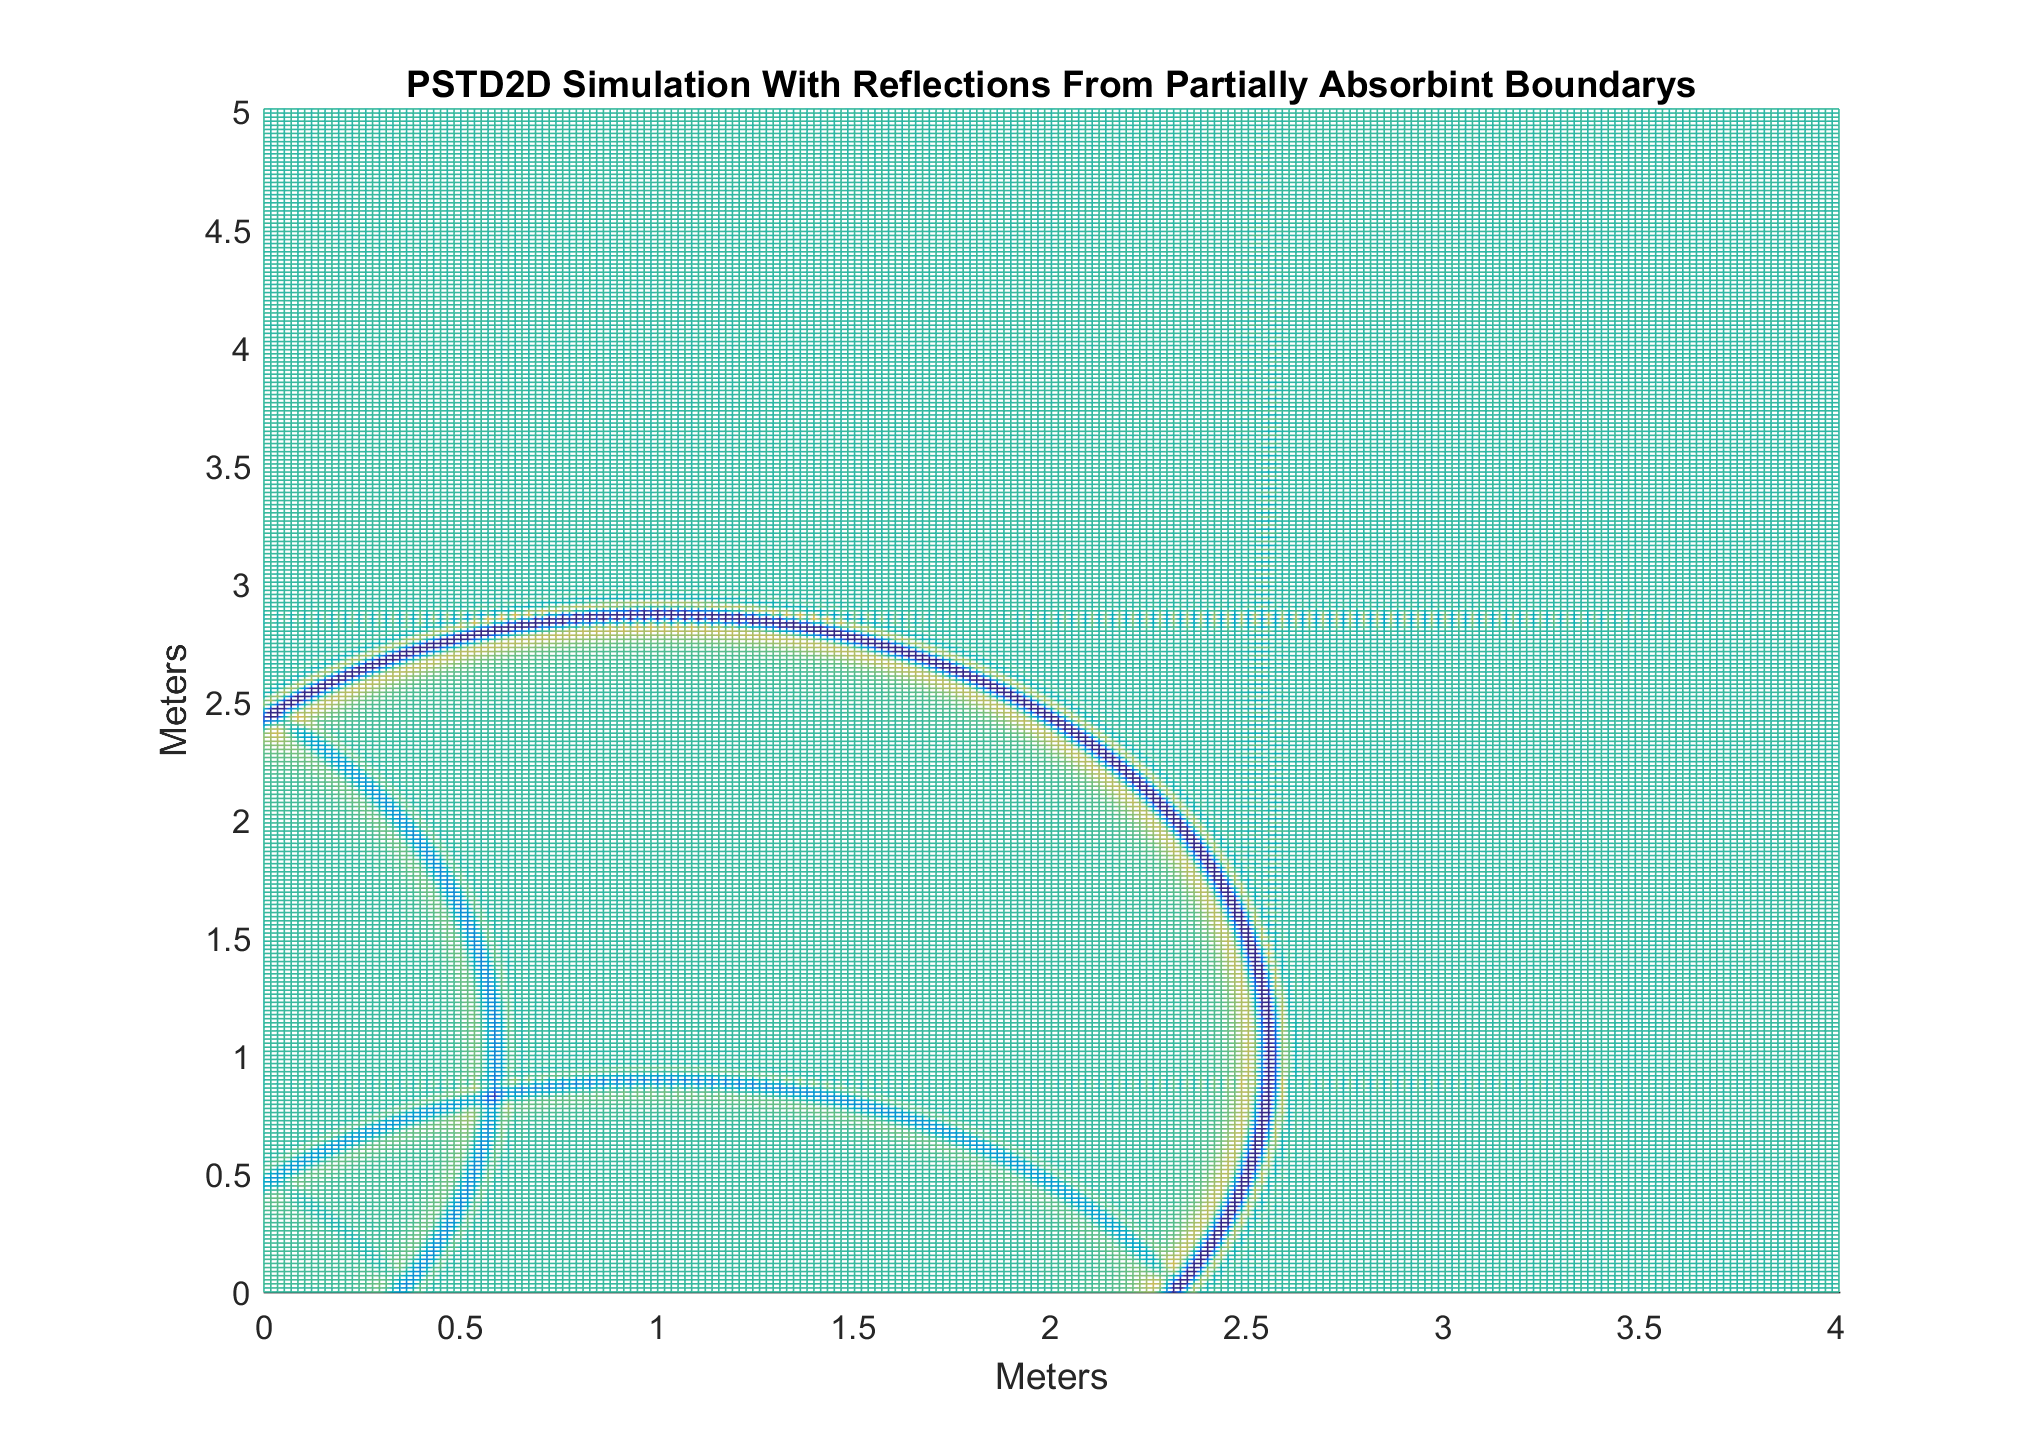
\includegraphics[width=0.75\textwidth]{./graphics/pstd2dwithreflectingboundaries.png}
  \caption{Example Plot of a 2D PSTD Simulation With Reflections}
\end{figure}

%\section{Validation: A 3D Simulation with empirical partially absorbing boundary conditions}
%\label{sec:3}
% Always give a unique label
% and use \ref{<label>} for cross-references
% and \cite{<label>} for bibliographic references
% use \sectionmark{ }
% to alter or adjust the section heading in the running head
%Instead of simply listing headings of different levels we recommend to let every heading be followed by at least a short passage of text. Furtheron please use the \LaTeX\ automatism for all your cross-references and citations.
\section{Sound Source Terms}
There are three main sound source excitation strategies in FDTD and PSTD simulations; hard, soft and transparent sources~\cite{Murphy2014}. Hard sources involve directly coupling a source signal to the pressure grid of a simulation, explicitly setting the pressure at a node for each time step of the simulation. This source type creates a discontinuity in the domain, that itself will cause incoming waves to reflect and diffract around it. This method also causes a shift in the frequencies of modal artifacts~\cite{Murphy2014}. A hard source maybe implemented using the following equation:\\
\begin{equation}
p_{xyz}^{t} = source^{t}\\
\end{equation}
Where the source is a function of time and is evaluated at points of $t$ up to $T$, and the points of $p_{xyz} are the points of excitation of the domain$.
A soft source such as the one used in this study for all three methods, imposes a pressure perturbation term to the newly calculated pressure at the point of interest in the pressure grid. This allows waves to pass the source location without being impeded by the source term itself. A soft source can cause an anomalous DC term to be added to the simulation, causing a spectral shift to occur as seen in the power spectral density plots of this report. Also a soft source excitation may be modulated by the error present in the simulation grid, as the source term is indirectly coupled to the domain and is modulated by any passing waves. A soft source may be implemented using the following equation:\\
\begin{equation}
p_{xyz}^{t} = p_{xyz}^{t} + source^{t}\\
\end{equation}
A transparent source involves applying error correction to the stimulus by convolving the impulse response of the simulation pressure grid with the source signal being applied to the domain, and taking the error from the original signal. This should correct for the error caused by the discretization and solving scheme, and allow for an accurate soft source coupling i.e. without causing extra reflections. This method does however exhibit the same dc term and spectral tilt inherent in the soft source. The impulse response of the domain can be taken by recording the incoming pressure at the source excitation point, when the source term is an ideal dirac function. A transparent source can be implemented using the following equation:\\
\begin{equation}
p_{xyz}^{t} = p_{xyz}^{t} + source^{t} - \Sigma_0^T h_{xyz}^{t = 0 : t}*source^{t = 0 : t}\\
\end{equation}


